% Hadron-Hadron Scatteing
%%%%%-------PROVA-------------
%\documentclass[12pt]{report}
%\usepackage[british]{babel}
%\usepackage{amsmath}
%\usepackage{amsfonts}
%\usepackage{amssymb}
%\usepackage{geometry}
%\geometry{hmargin={2cm,2cm},vmargin={2cm,2cm}}
%\usepackage{caption}
%\captionsetup{format=hang}
%\usepackage{graphicx}
%\usepackage{enumitem}
%\usepackage{float}
%
%
%
%\usepackage[colorlinks=true, linkcolor=blue]{hyperref} %to use autoref
%%%%%-------------------------

%\begin{document}


\chapter{Hadron-Hadron Scattering}

In a high energy proton-proton collision we can have either soft or hard processes. Most of the time the hard processes are accompanied by soft interaction, occurring along the hadron interaction.
The hard processes are well understood using perturbation theory, meanwhile the soft processes are not so well understood in fact these processes are described by non perturbative QCD. 

\section{QCD factorization theorem}

The factorization theorem was introduced first by Drell and Yan (ref: S.D. Drell and T.M. Yan, Ann. Phys. 66 (1971) 578.).

The hadron-hadron scattering is describe in terms of partons extending the formalism used for deep inelastic scattering. 
\begin{equation}
\sigma_{AB}=\displaystyle\int dx_a\,dx_b\,f_{a/A}(x_a)\,f_{b/B}(x_b)\,\hat{\sigma}_{ab \rightarrow X}
\label{eq:factorization1}
\end{equation}
Where X is a partonic/leptonic state and $a\,(b)$ a quark or an antiquark in the hadron $A\,(B)$. This is valid in the "scaling" limit:
\begin{equation}
	s\ \longrightarrow\ \infty \qquad\qquad\qquad \frac{M_X}{s}=\text{finite}
\end{equation}
The problem arise from the perturbative corrections from real and virtual gluon emission. This contribution give a logarithmic divergence (spoil the convergence of the perturbative expansion). These dependencies can be absorbed by the parton distribution function (DGLAP equations). This result in the violation of scaling:
\begin{equation}
	f_{a/A}(x_a)\ \longrightarrow\ f_{a/A}(x_a, Q^2)
\end{equation}  
Now the parton distribution function depend on the momentum scale $Q^2$. 

So, we can rewrite the factorization theorem in \eqRef{eq:factorization1} as:
\begin{equation}
	\sigma_{AB}=\displaystyle\int dx_a\,dx_b\,f_{a/A}(x_a,Q^2)\,f_{b/B}(x_b,Q^2)\,\hat{\sigma}_{ab \rightarrow X}
\label{eq:factorization2}
\end{equation}

Now the \emph{finite} corrections in the perturbative expansion are specific for each process (not universal). This leads in the \eqRef{eq:factorization2} to the $\alpha_s$ series:
\begin{equation}
	\sigma_{AB}=\displaystyle\int dx_a\,dx_b\,f_{a/A}(x_a,\mu_F^2)\,f_{b/B}(x_b,\mu_F^2)\,\left[\hat{\sigma}_0+\alpha_s(\mu_R^2)\hat{\sigma}_1+\dots\right]
\label{eq:factorization3}
\end{equation}
In \eqRef{eq:factorization3} two scales enter the formula:
\begin{itemize}
	\item[--] The \textit{factorization scale} $\mu_F$: this scale separates long- and short- distance.
	\item[--] The \textit{renormalization scale} $\mu_R$: the scale at which is evaluated the strong coupling $\alpha_s$.  
\end{itemize}

The higher-order corrections eliminate the cross section prediction dependencies on $\mu_R$ and $\mu_F$.
Typically, the scales are assumed to be equal.
For example in the Drell-Yan process the standard choice is $\mu_F=\mu_R=M$, with $M$ the lepton pair mass. 

The parton distribution functions used in the hard scattering are solution of the DGLAP (Dokshitzer–Gribov–Lipatov–Altarelli–Parisi) equation:

\begin{equation}
	\mu_F^2\frac{\partial f_{i/H}(x,\mu_F^2)}{\partial\mu_F^2}=\displaystyle\sum_j\frac{\alpha_s(\mu_F^2)}{2\pi}\displaystyle\int_x^1 \frac{dz}{z}\, P_{i\,\rightarrow\,j}(z)\ f_{j/p}\left(\frac{x}{z},\mu_F^2\right)
\end{equation}

Where $P_{i\,\rightarrow\,j}$ are the splitting functions: they are the probability to have a parton of type $i$ that became, by the emission of a quark or a gluon, a parton $j$, carrying fraction $z$ of the momentum of $i$.

The splitting functions have perturbative expansions: 
\begin{equation}
	P_{i\,\rightarrow\,j}(x,\alpha_s)=P_{i\,\rightarrow\,j}^{(0)}(x)+\frac{\alpha_s}{2\pi}P_{i\,\rightarrow\,j}^{(1)}(x)+\dots
\end{equation}

This procedure has been used to calculate Standard Model cross section in $p\overline{p}$ and $pp$ scattering respectively at Tevatron and LHC energies as shown in \figRef{figure:StandardModelCrossSections}.

\begin{figure}[!ht]
	\centering 
	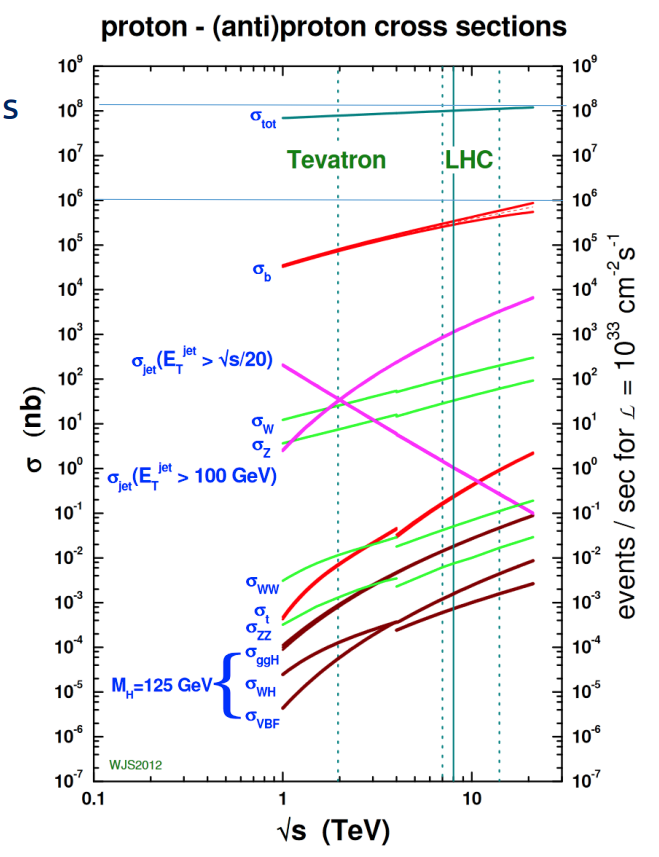
\includegraphics[width=12cm]{img/StandardModelCrossSections_color.png}
	\caption{Next-to-leading order cross sections at Tevatron and LHC colliders energies (the splitting are at the transition between $p\overline{p}$ and $pp$ cross section). Figure from (S. Catani, hep-ph/0005233)}
	\label{figure:StandardModelCrossSections}
\end{figure}

The parton distribution functions dependence on $Q^2$ can be derived theoretically via the DGLAP equations. While, the $x$ dependence is given fitting the deep-inelastic and other hard-scattering processes experimental data.
The experimental coverage in $(x,Q^2)$-plane is shown in \figRef{figure:xQ2planeCoverage} 
where is also underlined the relationship between $(x,Q^2)$ and kinematic variables in Drell-Yan processes for a final state with invariant mass $M$ and rapidity $y$ is shown. Assuming that the factorization scale $Q$ is equal to $M$ (The reference center of mass energy is $13\ \mathrm{TeV}$). So, for two incoming particles with four-momentum respectively $p_1$ and $p_2$ the relations with $y$ and $M$ are:  
\begin{equation}
	\begin{aligned}
		&p_1^\mu=\frac{\sqrt{s}}{2}(x_1,0,0,x_1)\\
&p_2^\mu=\frac{\sqrt{s}}{2}(x_2,0,0,-x_2)
	\end{aligned} \quad\Longrightarrow\quad x_1=\frac{M}{\sqrt{s}}e^y\qquad x_2=\frac{M}{\sqrt{s}}e^{-y}
\end{equation}
where  $s=(p_1^\mu+p_2^\mu)^2$.


\begin{figure}[!ht]
	\centering 	
	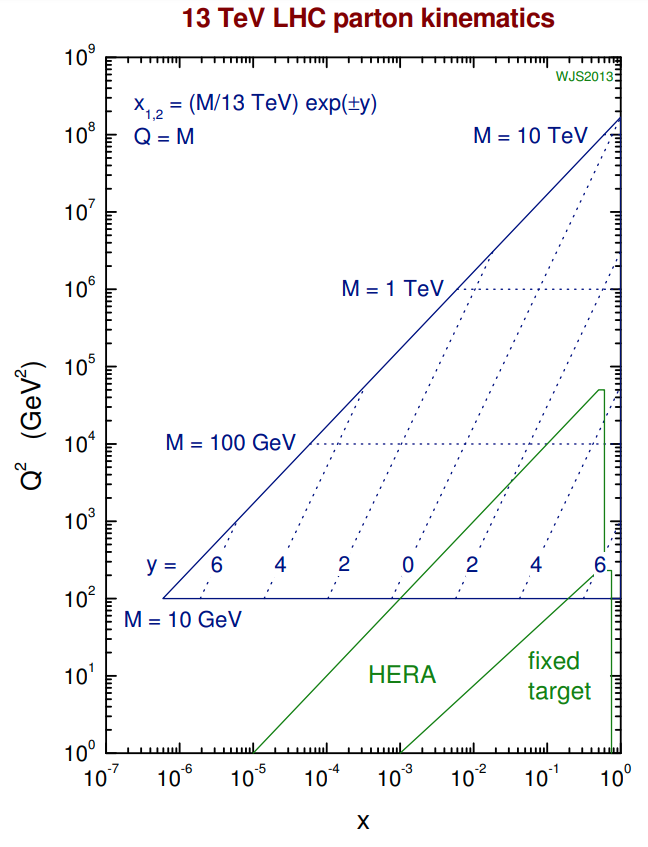
\includegraphics[width=12cm]{img/xQ2planeCoverage.png}
	\caption{Graphical representation of the parton $(x,Q^2)$ variables coverage of different experiments. For LHC these $x$ and $Q^2$ are related to the kinematic variables $y$ and $M$}
		\label{figure:xQ2planeCoverage}
\end{figure}

\section{Partonic cross section}

Partonic cross section is one of the fundamental ingredients in our recipe. This can be calculated in a perturbative series in $\alpha_s$ from QCD first principles using quantum field theory.

The calculation at the leading order (LO) is performed evaluating all the possible tree-level Feynman diagrams for every process. Evaluating the squared matrix element and integrating over the available phase space (analytically or numerically).

Already, here we can encounter some divergence that have to be avoided imposing restriction on the phase space.

\subsection{Higher order calculations}

The LO calculation can describe broad feature of a particular process and provide a first estimation of its cross section but in many cases this is insufficient.

The main source of uncertainty derives from the LO dependence  on the unphysical renormalization and factorization scales. Some process may contribute only when going beyond the first approximation, and some divergence can be resummed. 

To the next-to-leading orer (NLO) calculation participate all the Feynman diagrams that take an extra $\alpha_s$. This contribution can arise in two different way:
\begin{itemize}
	\item Virtual: internal lines (loops);
	\item Real: external lines (real particles).
\end{itemize}

Virtual corrections contains infrared divergences, arising from the integral on the loop circulating momentum, that cancel against infrared singularities given by collinear emissions or soft emissions. 

A common strategy for the rinormalization is dimensional regularization: consists into perform the calculation in a $D=4-2\epsilon$-dimensional space ($\epsilon<0$), in that way the singularities appear as single and double poles in $\epsilon$. Than, the limit $\epsilon\rightarrow0$ is taken after the divergences have cancelled.

This NLO calculation with regularization allows to extend the treatment to zero transverse momentum.

The importance of higher order calculations can be seen with the following example. In a $Z$ boson production:
\begin{enumerate}[label=$\arabic*)$]
	\item \textbf{LO}: the $Z$ is produced without transverse momentum ($p_T$), anything can recoil against the $Z$ for momentum conservation.
	\item \textbf{NLO}: the $Z$ acquire a finite $p_T$, in this case the $Z$ boson $p_T$ is balanced by a single \mbox{parton/gluon}.
	\item  \textbf{NNLO}: the $Z$ $p_T$ can be balanced by two jets. 
\end{enumerate}



Another important benefit of performing a NLO calculation is the the reduction of the dependence on the unphysical renormalization ($\mu_R$) and factorization ($\mu_F$) scales.
It is proven that higher order calculations is that observables calculated to order $\alpha_s^{\,n}$ are dependent on the unphysical scales only at order higher than $\alpha_s^{\,n+1}$. The range of predictions corresponding to different scale choices is usually attributed to \textit{theoretical uncertainties}.

\section{Parton Showers}

A different approach, instead than calculating order by order in the perturbative expansion, is to use an \textit{all-order} approach in order to describe the phenomena observed at high-energy colliders. 

different all-order approaches exist e.g. resummation and parton showers. Resummation is based on the observation that in many quantities the smallness of the expansion coefficients $\alpha_s$ is violated by large logarithmic enhancements. This take the dominant contribution from each order and "resum" them by means of an evolution equation. 
The main problem in QCD is related to the fact that lot of quantities have correction of the form $\alpha_s^n\log^k(Q_i/Q_j)$ where $Q_i$ and $Q_f$ are two different energies scales, for example:
\begin{itemize}
	\item[--] Renormalization and factorization scales logs: $\alpha_s^n\log^n(Q^2/\mu_f)$
\end{itemize}
Various methods to perform this resummation exist.

%%%% GRAPH on pT Z with effect of resummation 

An other \textit{all-order} approach is parton showers, this is implemented in different programs  \textsc{pythia}, \textsc{herwig} and \textsc{sherpa}. This start from few parton arising from hard interaction and than these are related to partons to a lower energy scale close to $\Lambda_{QCD}$ using the DGLAP evolution equation formalism, the solution at this equation can be write using a Sudakov form factor arising from the probability of no gluon emission in the evolution from higher scale to lower scale.




An example is the $Z$ production $p_T$ spectrum shown in \figRef{figure:pT_Z_CDF}. A comparison between experimental CDF data and theoretical predictions is shown: in the low $p_T$ region the \textit{all-order} approach regularize the divergence of the fixed order calculation and describe the data better then the last one. 

\begin{figure}[!ht]
	\centering
	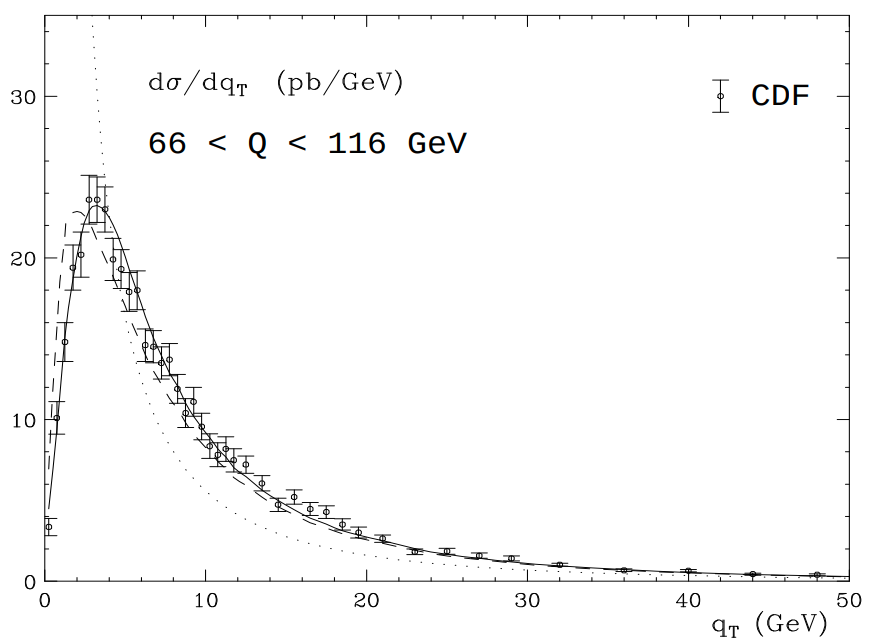
\includegraphics[width=12cm]{{img/pT_Z_CDF.png}}
	\caption{CDF data on $Z$ production cross section at Tevatron collider, CDF experiment, the predictions from fixed order calculation (dotted) with resummation (dashed), and with the inclusion of power corrections (solid) are compared (preso da A. Kulesza et al., hep-ph/0207148)}
	\label{figure:pT_Z_CDF}
\end{figure}



\bigskip
\bigskip
%%% ---



%In a \textbf{proton-proton collision}, additionally to the main hard scattering that can be described performing Matrix Element calculations (MEs) , also other scattering processes are possible. To well understood the proton-proton collision we need to describe other processes, besides to the hard scattering, that can underlying to this  \textbf{Multi Parton Interaction} (MPI) and the \textbf{Beam-Beam Remnants} (BBR).




%\end{document}